\documentclass{article}
\usepackage[preprint]{neurips_2026}

\usepackage[utf8]{inputenc}
\usepackage[T1]{fontenc}
\usepackage{hyperref}
\usepackage{url}
\usepackage{booktabs}
\usepackage{amsfonts}
\usepackage{amsmath}
\usepackage{microtype}
\usepackage{xcolor}
\usepackage{graphicx}

% This is an ES 678 course paper, not a conference submission.
\makeatletter
\renewcommand{\@noticestring}{ES 678 Course Project}
\makeatother

% Every number in the paper comes from results/tables; see SUPPLEMENTARY.md in the repository.
\newcommand{\todo}[1]{\textcolor{red}{[#1]}}

\title{Predicting Earthquake Damage to Buildings from Construction Attributes and Ground Shaking}

\author{%
  Abhishek Anand \\
  Roll Number: 24210004 \\
  ES 678, Indian Institute of Technology Gandhinagar
}

\begin{document}
\maketitle

\begin{abstract}
Fragility curves estimate earthquake damage from a building's structural type and the shaking at its site. We ask
whether machine-learning models that also see pre-earthquake building attributes do better in places they were not
trained on. Using 762,094 buildings surveyed after the 2015 Gorkha earthquake and peak ground acceleration (PGA)
from USGS ShakeMaps, we selected models by cross-validation over whole municipalities and tested them once, after
freezing every choice, on a held-out district of 98,019 buildings. A gradient-boosted model that starts from the
fragility curve and learns only a correction from building attributes improved the ranked probability score by
3\% on both ShakeMaps, in 13 and 12 of 13 test municipalities. Tree ensembles given PGA directly showed no
reliable gain, though a random split made them look far better.
\end{abstract}

\section{Problem and Motivation}
After a damaging earthquake, the first building-level loss estimates come from fragility curves: for each
structural type, a curve gives the probability of each damage grade at a given level of shaking, and nothing else
about the building enters. The 2015 Gorkha survey records much more, and it has become a popular machine-learning
benchmark with micro-F1 scores near 0.75 \citep{drivendata}. Most of that work splits buildings at random and uses
location codes as features, which rewards remembering how badly each place was hit and is of little use in the
next earthquake. Our question is narrower: \emph{do models that use pre-earthquake attributes with PGA predict
damage-grade probabilities, in municipalities and districts left out of training, more accurately than fragility
curves that use structural type and PGA alone?} We treat this as a hypothesis in which either answer is useful. If
the attributes help, inventories should record them; if they do not, structural type and shaking are enough, and
a detailed survey is not needed for prediction. One row is one building, and the prediction is one that could be
made within hours of an event, from an inventory and a ShakeMap, before any survey.

\section{Data and Preparation}
The Government of Nepal's post-earthquake survey \citep{nepaldata} covers 762,094 graded buildings in 11 districts
and 110 municipalities (grade shares 11/11/17/23/38\% in the ten development districts). We dropped 12 ungraded
rows, treated 3,144 ages coded 995 or more as missing, and flagged but kept the 1.3\% of records with
contradictory or implausible entries. The inputs are the 22 attributes known before the earthquake: storeys, age,
plinth area, height, slope, position, plan shape, foundation, roof and floor types, and 11 non-exclusive
superstructure flags. Fields recorded afterwards are excluded because they contain the answer: all 261,353
buildings with zero storeys after the event are grade 5. Shaking is the mean ShakeMap PGA \citep{shakemap} within
each municipality's boundary \citep{boundaries}, with all 110 matched. USGS has two maps of this event, the
automatic 2020 Atlas re-run (median municipal PGA 0.58\,g) and the reviewed 2015 NEIC map
(0.30\,g), and they rank municipalities differently (Spearman 0.72). We could not justify choosing one, so we
report both. For the fragility curves each building gets one of 9 structural types by material precedence, with
a separate class for strong-plus-weak mixes. Kavrepalanchok (98,019 buildings, 13 municipalities) was set aside
as the test district before any analysis, on size and grade mix alone, and locked in code. Every learned step,
including the fragility fits, is fitted on training folds only.

\section{Methods}
The baseline that matters is a set of \emph{fragility curves}: an ordered probit in $\ln\text{PGA}$, fitted by
maximum likelihood \citep{baker2015} for each structural type $c$,
\begin{equation}
P(\text{DG}\ge k \mid \text{PGA}, c)=\Phi\big((\ln \text{PGA}-\ln\theta_{c,k})/\beta_c\big),\quad k=2,\dots,5,
\end{equation}
where $\Phi$ is the standard normal CDF, $\theta_{c,2}<\dots<\theta_{c,5}$ are median PGAs and $\beta_c$ is one
dispersion per type; grade probabilities are differences of consecutive curves. A majority-class model is the
trivial baseline. Against these we compare four models that see all attributes, the type and $\ln$PGA: a ridge
ordinal logit, a shallow decision tree, a random forest and LightGBM \citep{ke2017}. Validation showed that trees
split municipal PGA finely enough to identify municipalities (Sec.~\ref{sec:depth}), so we built a fifth model, the
\emph{hybrid}, in which the fragility curve carries PGA and the trees see building attributes only:
\begin{equation}
P(\text{DG}=k\mid x)\propto \exp\big(\ln p^{\text{frag}}_k(\text{PGA},c)+f_k(x_{\text{attr}})\big),
\end{equation}
with $p^{\text{frag}}$ fitted on the training rows and $f_k$ boosted trees. Hyperparameters come from small grids
fixed in advance, LightGBM stops early on 15\% of the training municipalities, and we used no class weighting,
since the metrics judge probabilities.

\section{Evaluation Design}
We select models by 5-fold cross-validation over whole municipalities (97 in the development districts), repeated
with 3 fold assignments; for each model and map the setting with the lowest mean RPS wins. Two other designs are
checks that never influence selection: leave-one-district-out (LODO, 10 folds), which mimics the test, and a
random split of buildings, to show how optimistic it is. Before the test district was read, we froze the list of
runs and the rule for claiming a result, with SHA-256 hashes of the code and selection tables; the test was then
scored once. The main metric is the ranked probability score \citep{epstein1969},
$\text{RPS}_i=\frac{1}{4}\sum_{k=1}^{4}(F_{ik}-O_{ik})^2$, where $F_{ik}$ and $O_{ik}$ are the predicted and
observed cumulative probabilities of grade $\le k$; it respects grade order, and lower is better. We also report
the Brier score of $P(\text{DG}\ge4)$, log loss, quadratic weighted kappa (QWK) and accuracy, and all comparisons
are paired. On the test, we claim an improvement only if the mean paired $\Delta$RPS is negative and its 95\%
cluster-bootstrap interval over the 13 municipalities excludes zero.

\section{Results and Error Analysis}
\begin{figure}[t]
  \centering
  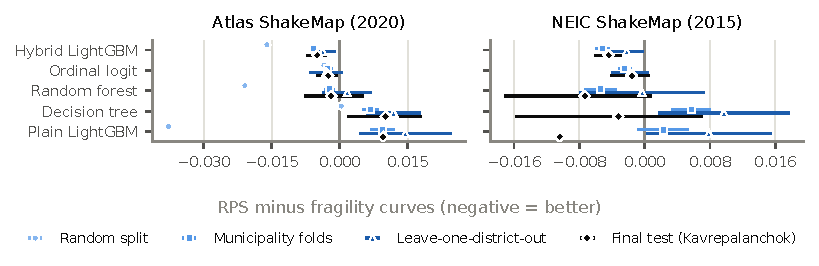
\includegraphics[width=\textwidth]{figures/14_fig1_gain_by_design.pdf}
  \caption{Paired RPS difference from the fragility curves (negative = better). Bars: mean $\pm1.96$ SE over
  folds (approximate); 95\% cluster bootstrap for the test. Random split: Atlas map only; plain LightGBM on
  the test: point only.}
  \label{fig:design}
\end{figure}
\begin{table}[t]
  \caption{Final test on Kavrepalanchok. $\Delta$RPS: paired difference from the same map's fragility curves
  [95\% cluster-bootstrap interval], municipalities better out of 13. Bold: lowest RPS of the map.}
  \label{tab:test}
  \centering
  {\footnotesize\setlength{\tabcolsep}{3.5pt}\begin{tabular}{@{}llrrrrrl@{}}
\toprule
Map & Model & RPS & Brier$_{\geq 4}$ & Log loss & QWK & Acc. & $\Delta$RPS vs fragility [95\% CI] \\
\midrule
Atlas & Majority class & 0.1744 & 0.2539 & 1.575 & 0.000 & 0.243 & -- \\
Atlas & Fragility curves & 0.1494 & 0.2378 & 1.425 & 0.431 & 0.323 & -- \\
Atlas & Decision tree & 0.1596 & 0.2456 & 1.483 & 0.394 & 0.311 & $+0.0102$ [$+0.0018$, $+0.0181$], 3/13 \\
Atlas & Random forest & 0.1476 & 0.2352 & 1.414 & 0.440 & 0.334 & $-0.0018$ [$-0.0077$, $+0.0052$], 8/13 \\
Atlas & Ordinal logit & 0.1469 & 0.2325 & 1.419 & 0.437 & 0.326 & $-0.0025$ [$-0.0051$, $-0.0004$], 10/13 \\
Atlas & Hybrid LightGBM & \textbf{0.1445} & 0.2316 & 1.394 & 0.450 & 0.342 & $-0.0049$ [$-0.0074$, $-0.0030$], 13/13 \\
\midrule
NEIC & Fragility curves & 0.1430 & 0.2280 & 1.388 & 0.415 & 0.326 & -- \\
NEIC & Decision tree & 0.1398 & 0.2224 & 1.375 & 0.514 & 0.381 & $-0.0032$ [$-0.0158$, $+0.0070$], 4/13 \\
NEIC & Random forest & \textbf{0.1357} & 0.2180 & 1.346 & 0.501 & 0.371 & $-0.0073$ [$-0.0171$, $+0.0009$], 8/13 \\
NEIC & Ordinal logit & 0.1415 & 0.2243 & 1.387 & 0.438 & 0.328 & $-0.0015$ [$-0.0042$, $+0.0006$], 9/13 \\
NEIC & Hybrid LightGBM & 0.1386 & 0.2230 & 1.359 & 0.461 & 0.349 & $-0.0044$ [$-0.0062$, $-0.0029$], 12/13 \\
\bottomrule
\end{tabular}
}
\end{table}
\textbf{The evaluation design decides the conclusion} (Fig.~\ref{fig:design}). On a random split the tree
ensembles look far ahead of the fragility curves (random forest $-0.021$, plain LightGBM $-0.038$ RPS). On new
districts the same models gain nothing or lose, and the random forest keeps only a small gain ($-0.002$ to
$-0.005$) on new municipalities. LODO anticipated the test (hybrid 0.1425 against 0.1445, Atlas map), whereas
municipality folds were optimistic by about 0.01.
\textbf{Final test} (Table~\ref{tab:test}). The hybrid beats the fragility curves on both maps, by 0.0049 and
0.0044 RPS (3\%), in 13 and 12 of 13 municipalities. The ordinal
logit gains about half as much and meets the claim rule only on the Atlas map. The random forest has the
lowest RPS on the NEIC map, but its interval includes zero, so we do not claim it.
\textbf{Where the models are wrong.} The gain is concentrated in minority building types and at the extremes of
storeys and age (hybrid on LODO: cement-mortar masonry $-0.018$, one storey $-0.010$); stone masonry, 80\% of the
stock, gains only 0.003, because its fragility curve already describes the typical house. The largest errors,
however, are district-wide and shared: every selected model over-predicts severe damage in Kavrepalanchok
(0.62--0.67 against 0.54; Fig.~\ref{fig:interp}c). The Atlas map gives this district the second-highest PGA
of the 11, and on that map the models without PGA scored best (RPS 0.139), which points to the shaking input.

\section{Graduate Depth Analysis}\label{sec:depth}
\begin{figure}[t]
  \centering
  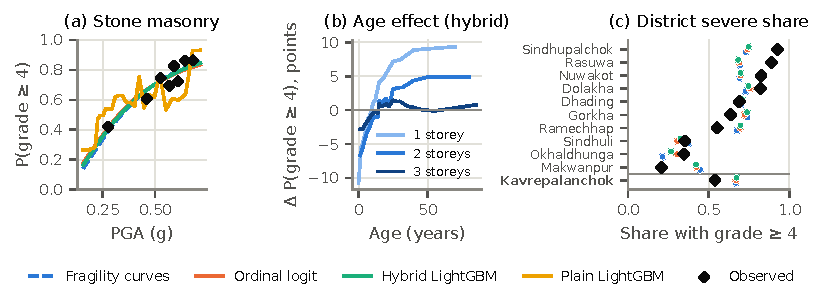
\includegraphics[width=\textwidth]{figures/14_fig2_interpretation.pdf}
  \caption{Atlas map. (a) P(grade $\ge 4$) against PGA implied by each model for stone masonry; diamonds are
  observed shares. (b) Accumulated local effect \citep{apley2020} of age on the hybrid's P(grade $\ge 4$), by
  storeys. (c) Predicted (dots, colours as in a) and observed severe share by district (LODO; test for
  Kavrepalanchok).}
  \label{fig:interp}
\end{figure}
\textbf{Information or flexibility?} Given only structural type and PGA, the ordinal logit matches the fragility
curves ($+0.0008$ RPS on municipality folds), while the random forest ($+0.024$) and LightGBM ($+0.018$) are much
worse; adding the attributes makes the ordinal logit better ($-0.0026$). So the gain comes from the attributes,
and flexibility alone hurts. The fragility curve that LightGBM implies is jagged and not even monotone
(Fig.~\ref{fig:interp}a), while the hybrid's type-average curve coincides with the fitted one, so its gain comes
from separating buildings within a type.
\textbf{Which inputs matter.} Refitting without one input group at a time shows how sensitive the prediction is
to each. For the ordinal logit, removing PGA costs 0.010--0.014 RPS on municipality folds, against at most 0.0007
for any group of building attributes. In the hybrid, where the curve carries PGA, age matters most (0.0016), then
foundation, superstructure, roof and storeys (0.0003--0.0009). Six groups (ground-floor type, height, slope, plan
shape, plinth area, position) add under 0.0002 each. \emph{Verdict for future inventories:} PGA, structural type
and materials, storeys, age, foundation, roof and upper-floor type carry the signal. With only these, the ordinal
logit barely changes on the test district, but the hybrid keeps only 55--77\% of its gain, so the six minor
inputs are worth recording when they are cheap. The response is not linear: accumulated local effects, applied as in
\citet{borah2026}, show that a third storey adds about 8 points to the probability of severe damage, and that age
matters by 20 points for one-storey buildings but only 4 for three-storey ones (Fig.~\ref{fig:interp}b).
\textbf{Calibration.} On new districts the ML models are better calibrated than the fragility curves
(calibration error 0.017--0.028 against 0.035--0.063).
\textbf{Where the error sits.} Of the hybrid's severe-damage Brier score, 10\% is district-wide, 8\%
municipality-wide, 8\% ward-wide and 74\% lies between buildings of the same ward. Without surveyor IDs, we used \emph{twins}, buildings in the same ward with identical values
of all 22 attributes; they receive the same grade in only 61\% of pairs. A model that
knew each twin group's own grade distribution would score RPS 0.070; the hybrid scores 0.127.

\section{Limitations and Conclusion}
We use one earthquake and one test district, which borders development districts. District-wide offsets of
0.1--0.2 in severe share, likely ShakeMap error, dominate the error. Sec.~\ref{sec:depth} is post hoc and associational. Only LightGBM was combined
with the fragility curve; an ordinal logit with a fragility offset, or LightGBM with a monotone PGA constraint,
might do better. A stronger claim needs a second earthquake and recorded shaking. Building attributes improve on
fragility curves in unseen districts, modestly (3\% RPS) and only when PGA enters smoothly. Correcting a
fragility curve works; replacing it does not.

\section{Reproducibility and AI-Use Disclosure}
Code and supplementary material (all result tables and figures; index in \texttt{SUPPLEMENTARY.md}):
\url{https://github.com/AnKehsih/Building-Fragility-Curve-Using-ML}. Data: CC0 survey \citep{nepaldata}, public-domain
USGS ShakeMaps \citep{shakemap}, CC BY-SA boundaries \citep{boundaries}. Software:
scikit-learn \citep{pedregosa2011}, LightGBM \citep{ke2017}. \textbf{AI use.} Claude Code (Anthropic) wrote and debugged the code, cleaned the data, and helped design the figures. Meanwhile, the author formulated the research question, selected the methodology, and made all key modeling decisions. The AI did not generate any final conclusions.

\begin{thebibliography}{10}
\setlength{\itemsep}{0pt}
\bibitem[Apley and Zhu(2020)]{apley2020}
D.~W. Apley and J.~Zhu. Visualizing the effects of predictor variables in black box supervised learning models.
\emph{J. R. Stat. Soc. B}, 82(4):1059--1086, 2020.
\bibitem[Baker(2015)]{baker2015}
J.~W. Baker. Efficient analytical fragility function fitting using dynamic structural analysis.
\emph{Earthquake Spectra}, 31(1):579--599, 2015.
\bibitem[Borah et~al.(2026)]{borah2026}
A.~Borah, A.~Datta, A.~S. Kumar, R.~Dave, and U.~Bhatia. Dense canopies reverse the cooling effect of urban
greening in humid cities. \emph{Nat. Commun.}, 17:5997, 2026.
\bibitem[CBS and NPC(2017)]{nepaldata}
Central Bureau of Statistics and National Planning Commission, Nepal. Household Registration for Housing
Reconstruction Survey, 2015 Nepal Earthquake Open Data Portal; Kaggle copy (CC0).
\bibitem[DrivenData(2019)]{drivendata}
DrivenData. Richter's Predictor: modeling earthquake damage.
\url{https://www.drivendata.org/competitions/57/nepal-earthquake/}.
\bibitem[Epstein(1969)]{epstein1969}
E.~S. Epstein. A scoring system for probability forecasts of ranked categories.
\emph{J. Appl. Meteorol.}, 8(6):985--987, 1969.
\bibitem[Ke et~al.(2017)]{ke2017}
G.~Ke et~al. LightGBM: a highly efficient gradient boosting decision tree. In \emph{NeurIPS 30}, 2017.
\bibitem[Open Data Nepal(2026)]{boundaries}
Open Data Nepal. Municipal boundaries of Nepal (CC BY-SA), opendatanepal.com, Nov 2026.
\bibitem[Pedregosa et~al.(2011)]{pedregosa2011}
F.~Pedregosa et~al. Scikit-learn: machine learning in Python. \emph{JMLR}, 12:2825--2830, 2011.
\bibitem[USGS(2020)]{shakemap}
U.S. Geological Survey. ShakeMap, event us20002926: Atlas v1 (2020), NEIC v9 (2015).
\end{thebibliography}

\end{document}
